\section{CALENR}
\label{sCALENR}

\hypertarget{sCALENRhy}{The}
CALENR\index{CALENR|textbf} module of NJOY is designed to produce
CALENDF probability tables from information recovered in a PENDF tape.
CALENDF probability tables are known as {\sl mathematical tables} and
are used in many deterministic lattice codes to represent the resonnant
behavior of cross sections \cite{ribon,calendf}. They are different from
PURR\index{PURR|textbf} tables in three different ways:
\begin{itemize}
\item CALENDF probability tables are used in both the resolved and unresolved
resonance ranges.
\item The number of weights and base points in each energy group is different
and carefully adjusted to reduce the size of tables.
\item They are written to the GENDF tape.
\end{itemize}

\subsection{Moment-based probability tables}
\label{ssCALENR_Theory1}
We first consider the lethargy variation of microscopic total cross section
and the corresponding probability density $\Pi(\sigma)$, as
represented in Fig.~\ref{fig:energy}, where

\vskip -0.5cm

\begin{description}
\item [$u=$] lethargy
\item [$\sigma(u)=$] microscopic total cross section
\item [$\Pi(\sigma) d\sigma=$] probability for the microscopic total cross
section of the resonant isotope, to have a value between $\sigma$ and
$\sigma+d\sigma$ in group $g$. Note that we have not explicitely indicated
the group $g$ dependence of $\Pi(\sigma)$.
\end{description}

As might be expected, the probability density $\Pi(\sigma)$ is normalized to
unity:

\begin{equation}
\int_{0}^{\max(\sigma)} d\sigma \, \Pi(\sigma)=1 \ \ \ .
\label{eq:eq3}
\end{equation}

\vskip 0.1cm

Using this definition, any Riemann integral in energy, with a
$\sigma$--dependent integrand, can be replaced by an equivalent Lebesgue
integral. The average value of an arbitrary function $f\left[ \sigma(u)\right]$
in group $g$ can be written as

\begin{equation}
{1 \over
\Delta u_g}\int_{u_{g-1}}^{u_g} du \; f\left[ \sigma(u)\right]=
\int_{0}^{\max(\sigma)} d\sigma \, \Pi(\sigma) \ f(\sigma)
\label{eq:eq3b}
\end{equation}

\noindent where $u_g=$ lethargy corresponding to the lower energy limit of
group $g$ and $\Delta u_g=u_g-u_{g-1}$. The probability density behaves as
$du/d\sigma$; its analytical value will therefore peak to infinity at each
cross section value such that $d\sigma(u)/du=0$, as represented in
Fig.~\ref{fig:energy}.

%
\begin{figure}[h!]
\centering
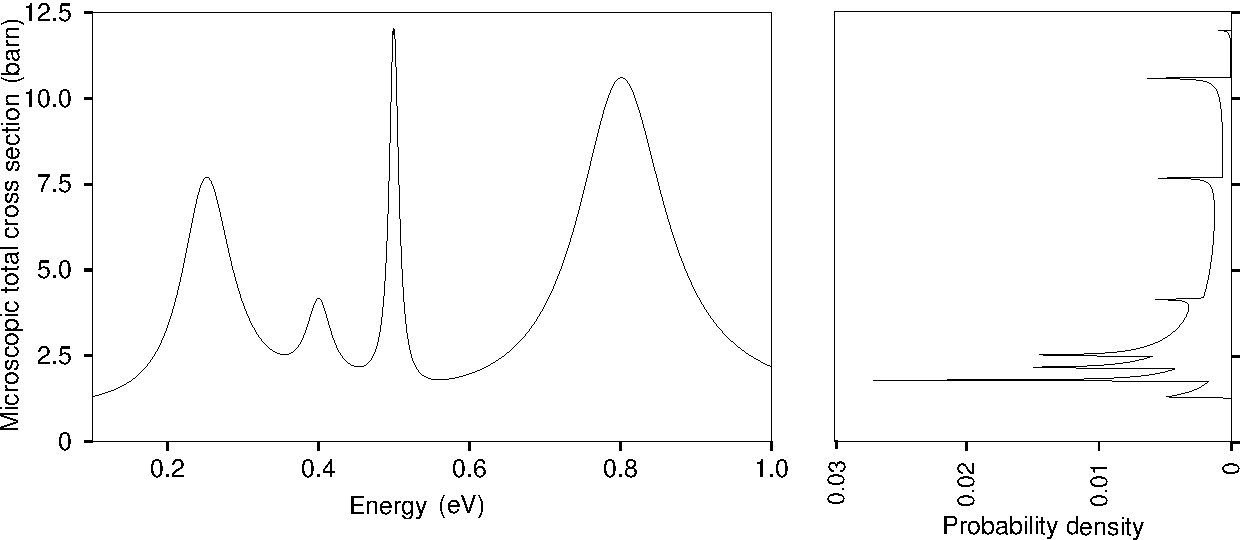
\includegraphics[scale=0.5]{figs/energy.pdf}
\parbox{11cm}{\caption{Representation of a probability density $\Pi(\sigma)$.}
\label{fig:energy}}
\end{figure}
%

\vskip 0.1cm

The probability density $\Pi(\sigma)$ is represented by a series of $K$ Dirac
distributions centered at discrete values $\sigma_k$ of the microscopic total
cross section for the resonant isotope. Each discrete level is called a
{\sl subgroup} and is also characterized by a discrete weight $\omega_k$. This
is equivalent to dividing the range of the total microscopic cross section in
group $g$ into $K$ intervals or bands and assigning a cross-section base point
$\sigma_k$ to each band. The probability density is written

\begin{equation}
\Pi(\sigma)=\sum_{k=1}^{K} \delta(\sigma-\sigma_k) \, \omega_k.
\label{eq:eq4}
\end{equation}

\noindent where

\begin{equation}
\sum_{k=1}^{K} \omega_k = 1 \ \ \ .
\end{equation}

\vskip 0.1cm

Substitution of Eq.~(\ref{eq:eq4}) into Eq.~(\ref{eq:eq3b}) leads to the
following discretization:

\begin{equation}
{1 \over
\Delta u_g}\int_{u_{g-1}}^{u_g} du \; f\left[ \sigma(u)\right]=\sum_{k=1}^{K}
\omega_k \, f(\sigma_k) .
\label{eq:eq4b}
\end{equation}

\vskip 0.1cm

The sets of values $\{ \omega_k, \ \sigma_k \ ; \ k=1,K \}$ corresponding to
energy group $g$ is called a probability table for the variable $\sigma$.

\vskip 0.1cm

The self-shielding method also requires information for {\sl partial} cross
sections $\sigma_\rho$ (e.g., for the scattering, absorption of fission cross
sections). An additional {\sl correlated base point} $\sigma_{\rho,k}$ is
defined for each partial cross section, so that any Riemann integral involving
this cross section could be written as

\begin{equation}
{1 \over \Delta u_g}\int_{u_{g-1}}^{u_g} du \; \sigma_\rho(u) \,
f\left[\sigma(u)\right]=\sum_{k=1}^{K} \omega_k \, \sigma_{\rho,k} \,
f(\sigma_k).
\label{eq:eq4c}
\end{equation}

\vskip 0.1cm

Again, we have not explicitely indicated the group $g$ dependence of the
various components in Eqs.~(\ref{eq:eq4c}).

\vskip 0.1cm

Mathematical probability tables are {\sl consistent}: The base points
$\sigma_k$ and $\sigma_{\rho,\ell}$ are constrained as follows:
$$\min(\sigma(u))\le\sigma_k\le\max(\sigma(u)) \ , \ \ \ \ \
\min(\sigma_\rho(u))\le\sigma_{\rho,\ell}\le\max(\sigma_\rho(u)) \ ,$$
the values of the probability table are real, and the weights are positive.

\vskip 0.1cm

The calculation of a mathematical probability table can be performed using the
moment--based approach, in which the position of the base points $\sigma_k$ and
values of the weights $\omega_k$ are simultaneously determined.
Here, the number of subgroups is much smaller, resulting in important savings
in CPU resources as compared to a multiband method. The saving is similar to
the one observed when we put a Gauss-Legendre quadrature in place of a
trapezoidal integration. This approach preserves the consistency of the
probability tables.

\subsection{The Ribon method}
\label{ssCALENR_Theory2}
\vskip 0.5cm

We first give an overview of the moment--based method, as implemented in the
CALENDF code. This method allows the calculation of a probability table in an
energy group $g$, using a straightforward transformation of the pointwise
information available in the PENDF file.

\vskip 0.1cm

Negative and positive moments of the total cross section are first computed
from the following Riemann integrals of the PENDF data:

\begin{equation}
{\cal M}_\ell={1 \over
\Delta u_g}\int_{u_{g-1}}^{u_g} du \; \sigma(u)^\ell .
\label{eq:eq6}
\end{equation}

These integrals are obtained as quadratures of PENDF continuous energy data in
the resolved resonance range and as Lebesgue quadratures of PURR probability
tables in the unresolved resonance range.

\vskip 0.1cm

A $K$--order probability table must be capable of preserving $2K$ selected
moments of Eq.~(\ref{eq:eq6}):

\begin{equation}
\sum_{k=1}^K \omega_k \ (\sigma_k)^\ell={\cal M}_\ell \  \ ; L_{\rm min}\le
\ell \le L_{\rm max}
\label{eq:eq7}
\end{equation}

Zeroth and first moments must always be preserved by the probability table in
order to satisfy the conservation relation for the weights and the value of the
infinite dilution total cross section. This imposes the following conditions:

\begin{equation}
\nonumber 2-2K \le L_{\rm min} \ \le \ 0 \ \ {\rm and}
\ \ L_{\rm max} = 2K+L_{\rm min}-1 \ \ .
\end{equation}

\vskip 0.1cm

In the moment--based approach, Ribon has chosen $L_{\rm min}=1-K$ and
$L_{\rm max}=K$ \cite{ribon}. Negative and positive moments help to preserve the
self-shielded reaction rate at low and high values of the resonant cross
section, respectively.

\vskip 0.1cm

Considering the Stieltjes generating function of total cross-section moments,
defined as a dimensionless quantity. We obtain

\begin{equation}
F(z)=\int_{0}^{\max(\sigma)} d\sigma \, \Pi(\sigma) \,
{\left(z\sigma\right)^{1-K} \over 1-z\sigma}=\sum_{\ell=1-K}^{K} z^\ell \,
{\cal M}_\ell \, + \, {\cal O}(z^{K+1}) \ \ .
\label{eq:eq8}
\end{equation}

\vskip 0.1cm

The right hand side of Eqs.~(\ref{eq:eq8}) will accurately represent low and
high values of the resonant cross section if we can force the error term
${\cal O}(z^{K+1})$ to vanish. Using a Pad\'e approximation to represent the
left hand side, the Stieltjes generating function can be written

\begin{equation}
z^{K-1} \ F(z)=\sum_{\ell=0}^{2K-1} z^\ell \, {\cal M}_{\ell-K+1}={a_0+a_1 \,
z+\ldots+a_{K-1}\ z^{K-1} \over b_0+b_1 \, z+\ldots+b_{K-1}\, z^{K-1}+z^K}
\label{eq:eq9}
\end{equation}

\noindent so that

\begin{equation}
\left(z^K+\sum_{k=0}^{K-1} b_k \, z^k\right) \left(\sum_{\ell=0}^{\ 2K-1} z^\ell
\, {\cal M}_{\ell-K+1}\right)=\sum_{k=0}^{K-1} a_k \, z^k \ \ \ .
\label{eq:eq9a}
\end{equation}

\vskip 0.1cm

We identify the coefficients of the powers of $z$ which are between $K$ and
$2K-1$. The coefficients $b_k$ are obtained as the solution of the following
linear system:

\begin{equation}
\left(\begin{matrix} {\cal M}_{K}  &{\cal M}_{K-1}&\ldots&{\cal M}_{1}\cr
         {\cal M}_{K-1}&{\cal M}_{K-2}&\ldots&{\cal M}_{0}\cr
         \vdots        &\vdots       &\ddots &\vdots      \cr
         {\cal M}_{1} &{\cal M}_{0}  &\ldots &{\cal M}_{2-K}\end{matrix}\right)
\left(\begin{matrix} b_0\cr b_1\cr \vdots \cr b_{K-1}\end{matrix}\right)=-
\left(\begin{matrix} {\cal M}_{0}\cr {\cal M}_{-1}\cr \vdots \cr {\cal M}_{1-K}
\end{matrix}\right) \ \ \ .
\label{eq:eq10}
\end{equation}

\vskip 0.2cm

A $L D L^\top$ factorization of the coefficient matrix is next performed.
The $b_n$ coefficients of Eq.~(\ref{eq:eq9}) are the components of
the solution of the $L D L^\top$ system and the base points of the probability
table are the roots of the following polynomial:

\vskip -0.2cm

\begin{equation}
\prod_{k=1}^K (z-\sigma_k)=b_0+b_1 \ z+\ldots+b_{K-1} \ z^{K-1}+z^K \ \ \ .
\label{eq:eq11}
\end{equation}

\vskip 0.1cm

Similarly, the coefficients $a_k$ could be obtained by identification of the
powers of $z$ which are between $0$ and $K-1$ in Eq.~(\ref{eq:eq9a}). However,
we have chosen to process in a different way.
The coefficients $a_k$ are not computed and the weights of
the probability table are computed directly, using the knowledge of the
base points, in such a way as to preserve selected moments
of the total cross section as defined in the discretized form of
Eq.~(\ref{eq:eq6}):

\begin{equation}
{\cal M}_\ell=\sum_{k=1}^{K}\; \omega_k \ \sigma_k^\ell \ \ \ .
\label{eq:eq11b}
\end{equation}

\vskip 0.1cm

In his work, Ribon has chosen to preserve {\sl all} the moments in the
interval $1-K\le \ell \le K$,
in a root-mean-square sense. We have modified the
original Ribon approach to gain numerical stability, avoiding the
calculation and $L D L^\top$ factorization of a normal matrix
$\left({\bf A}^\top{\bf A} \right)^{-1}{\bf A}^\top$, where ${\bf A}$ is a
transposed Vandermonde matrix.

\vskip 0.1cm

In the proposed approach, we have selected the moments in the interval
$-K/2\le \ell \le (K-1)/2$ to compute the $K$ weight values. Of course,
all these approaches are theoretically equivalent if we assume no rounding
error, as the number of unknowns ($2K$) is equal to the number of moments to
be preserved. In our work, the weights are computed as the solution
of the following linear system:

\begin{equation}
\left(\begin{matrix}   1 & 1 & \hspace{-0.5em}\ldots & 1 \cr
         \sigma_1 & \sigma_2 & \hspace{-0.5em}\ldots &
         \hspace{-0.5em}\sigma_K \cr
         \vdots   & \vdots   & \hspace{-0.5em}\ddots &
         \vdots   \cr
         \sigma_1^{K-1} &  \sigma_2^{K-1} & \hspace{-0.5em}\ldots
         & \hspace{-0.5em}\sigma_K^{K-1}\end{matrix}\right)
\left(\begin{matrix} \omega_1 \ (\sigma_1)^{k_0}\cr \omega_2 \,
(\sigma_2)^{k_0}\cr \vdots \cr \omega_K \, (\sigma_K)^{k_0}\end{matrix}\right)=
\left(\begin{matrix} {\cal M}_{k_0}\cr \hspace{-0.2em}{\cal M}_{k_0+1}\cr
\vdots \cr {\cal M}_{k_1}\end{matrix}\right)
\label{eq:eq12}
\end{equation}

\noindent where $k_0=-K/2$ and $k_1=(K-1)/2$.

\vskip 0.1cm

This linear system can be solved without pivoting, using the known analytical
inverse of a Vandermonde matrix. We obtain:

\begin{equation}
\omega_k={(-1)^{K-1} \ (\sigma_k)^{-k_0}\over \prod\limits_{\ell=1\atop \ell
\neq k}^K \left( \sigma_\ell-\sigma_k\right)}
\sum_{\ell=0}^{K-1} c_{k,\ell} \ {\cal M}_{k_0+\ell}
\label{eq:eq13}
\end{equation}

\noindent where $1\le k \le K$ and where $c_{k,\ell}$ is a coefficient of the
polynomial written as
\begin{equation}
c_{k,0}+c_{k,1} \ z+\ldots+c_{k,K-1} \, z^{K-1}=\prod\limits_{\ell=1\atop \ell
\neq k}^K (z-\sigma_\ell).
\label{eq:eq14}
\end{equation}

\vskip 0.1cm

Negative and positive {\sl partial moments} are next computed from the
following Riemann integrals of the PENDF data:

\begin{equation}
{\cal M}_{\rho,\ell}={1 \over \Delta u_g}\int_{u_{g-1}}^{u_g} du \;
\sigma_\rho(u) \, \sigma(u)^\ell.
\label{eq:eq15}
\end{equation}

\vskip 0.1cm

A $K$--order probability table must be capable of preserving $K$ selected
moments of Eq.~(\ref{eq:eq15}):

\begin{equation}
\sum_{k=1}^K \omega_k \, \sigma_{\rho,k} \ (\sigma_k)^\ell={\cal M}_{\rho,\ell}
\  \ ; L_{\rm min}\le \ell \le L_{\rm max}
\label{eq:eq16}
\end{equation}
\noindent where $L_{\rm min}=1-K/2$ and $L_{\rm max}=K/2$.

The correlated base points $\sigma_{\rho,k}$ are computed as the solution of
the following linear system:

\begin{equation}
\left(\begin{matrix} 1 & 1 & \hspace{-0.5em}\ldots & 1 \cr
         \sigma_1 & \sigma_2 & \hspace{-0.5em}\ldots &
         \hspace{-0.5em}\sigma_K \cr
         \vdots   & \vdots   & \hspace{-0.5em}\ddots &
         \vdots \cr
         \sigma_1^{K-1} & \sigma_2^{K-1} & \hspace{-0.5em}\ldots
         & \hspace{-0.5em}\sigma_K^{K-1}\end{matrix}\right)
\left(\begin{matrix} \omega_1 \, \sigma_{\rho,1} \, (\sigma_1)^{k_0}\cr \omega_2
\, \sigma_{\rho,2} \ (\sigma_2)^{k_0}\cr \vdots \cr \omega_K \, \sigma_{\rho,K}
\, (\sigma_K)^{k_0}\end{matrix}\right)=
\left(\begin{matrix} {\cal M}_{\rho,k_0}\cr \hspace{-0.2em}{\cal M}_{\rho,k_0+1}
\cr \vdots \cr {\cal M}_{\rho,k_1}\end{matrix}\right)
\label{eq:eq17}
\end{equation}

\vskip 0.1cm

This linear system can be solved without pivoting, using the known analytical
inverse of a Vandermonde matrix. We obtain:

\begin{equation}
\sigma_{\rho,k}={(-1)^{K-1} \ (\sigma_k)^{-k_0}\over \omega_k \,
\prod\limits_{\ell=1\atop \ell \neq k}^K \left( \sigma_\ell-\sigma_k\right)}
\sum_{\ell=0}^{K-1} c_{k,\ell} \ {\cal M}_{\rho,k_0+\ell} .
\label{eq:eq18}
\end{equation}

\vskip 0.1cm

For each resonant isotope and each resonant energy group, the probability
tables corresponding to different orders $K$ are obtained and their accuracy
is evaluated by computing Bondarenko self-shielded cross sections for a grid
of selected dilutions. The table with smallest order, meeting the accuracy
criteria, or the most accurate table, is selected. A maximum order of 12 is
allowed, but this order is seldom reached. There is no practical incentive
to allow a greater maximum order as high order tables may induce numerical
instabilities, overcoming potential increases in accuracy.

\subsection{User Input}
\label{ssCALENR_UserInp}

The following description of the user input is reproduced from
the comment cards at the beginning of the CALENR module.
\index{CALENR!CALENR input}
\index{input!CALENR}

\small
\begin{ccode}
   !---input specifications (free format)----
   !
   ! card 1 file units
   !   nendf   input endf unit
   !   npendf  input pendf unit
   !   nin     unit for input gendf tape
   !   nout    unit for output gendf tape
   !   ipreci  accuracy criterion for tables (=1/=2/=3/=4)
   !   iprint  long print option (0/1=minimum/maximum) (default=0)
   ! card 2
   !   matd    material to be processed
   !           matd=0 terminates calenr
   !   ntemp   no. of temperatures (default=1)
   ! card 3
   !   temp    temperatures in kelvin (including zero)
   ! card 4 energy limits for dilution-dependent xs data. This data
   !        is important to avoid self-shielding in very low and
   !        very high energy group xs and to reduce the size of the
   !        probability tables. (one card per material)
   !   eres0     lower limit of resolved resonance xs data (ev)
   !   eres1     upper limit of unresolved resonance xs data (ev)
   !
   !            repeat cards 2 to 4 for all materials desired
   !            matd=0/ terminates calenr run.
   !-----------------------------------------------------------------

\end{ccode}
\normalsize

The following sample run prepares a GENDF tape for Pu239.
The numbers on the left are for reference; they are not part of the input.

\small
\begin{ccode}
  1.   --
  2.   -- Pu239
  3.   --
  4.   moder
  5.    40 -21
  6.   reconr
  7.    -21 -22
  8.    'pendf tape from /tmp/endfb8r0'/
  9.    9437 1/
 10.    0.001  0.  0.005/
 11.    'Pu239 from /tmp/endfb8r0 at Thu Mar 26 16:01:52 2020' /
 12.    0/
 13.   broadr
 14.    -21 -22 -23
 15.    9437 2/
 16.    0.001/
 17.    2.930000E+02 5.500000E+02/
 18.    0/
 19.   purr
 20.    -21 -23 -24
 21.    9437 2 1 20 32/
 22.    2.930000E+02 5.500000E+02/
 23.    1.000000E+10/
 24.    0/
 25.   thermr
 26.    0 -24 -35
 27.    0 9437 16 2 1 0 0 1 221 0
 28.    2.930000E+02 5.500000E+02/
 29.    0.001 4.0
 30.   groupr
 31.    -21 -35 0 -26 0 0
 32.    9437 35 0 -4 1 2 1 1 0
 33.    'Pu239 from /tmp/endfb8r0 at Thu Mar 26 16:06:27 2020' /
 34.    2.930000E+02 5.500000E+02/
 35.    1.000000E+10/
 36.    677.2873 10.8897 20000 / Homog. Flux Calc.Param
 37.    0.2 0.0253 820.3e3 1.40e6 / iwt=4 parameters
 38.    3/
 39.    3 221 /
 40.    3 452 /
 41.    3 455 /
 42.    5 455 /
 43.    6 /
 44.    6 221 /
 45.    0/
 46.    3/
 47.    3 221 /
 48.    3 452 /
 49.    3 455 /
 50.    5 455 /
 51.    6 /
 52.    6 221 /
 53.    0/
 54.    0/
 55.   calenr
 56.    -21 -35 -26 -27 2 1/
 57.    9437 2 /
 58.    2.930000E+02 5.500000E+02 /
 59.    2.767920E+00 1.227734E+05 /
 60.    0/
 61.   moder
 62.    -27 51
 63.   stop
\end{ccode}
\normalsize

\subsection{Coding Details}
\label{ssCALENR_details}

The main entry point is subroutine \cword{calenr} exported by
module \cword{calenm}\index{modules!calenm@{\ty calenm}}.
The code begins by reading the user's input. It then locates the
position for the new material on the old GENDF\index{GENDF}
tape (if any) and copies the earlier results to the new output
tape. The desired material is also located on the input
PENDF\index{PENDF} tape prepared previously using
\hyperlink{sRECONRhy}{RECONR}\index{RECONR}.
A new material header is then written onto the output tape leaving
the code ready to begin the loop over seven reaction types:
\vskip 0.1cm
\begin{tabular}{| l | l |}
\hline
{\tt MT} code & reaction \\
\hline
1 & total cross section \\
2 & elastic scattering cross section\\
4 & inelastic scattering cross section\\
16 & (n,2n) cross section \\
17 & (n,3n) cross section \\
18 & fission cross section \\
102 & radiative capture cross section \\
\hline
\end{tabular}

\vskip 0.2cm

CALENR proceed in four steps. For each material and each temperature:
\begin{itemize}
\item Recover infinite dilution cross sections from the input GENDF tape for
the total and a list of six partial {\tt MT} reactions;
\item Recover the pointwise cross sections for these seven {\tt MT} reactions
from the input PENDF tape;
\item Recover PURR-type probability tables for the total, elastic scattering,
fission and capture reactions from the input PENDF tape;
\item Compute CALENDF probability tables for these seven {\tt MT} reactions and
store them on the output GENDF tape.

CALENDF probability table information is stored in seven {\tt MT} reactions
with new {\tt MF} $=$ 50 on the output GENDF tape:
\vskip 0.1cm
\begin{tabular}{| l | l |}
\hline
{\tt MT} code & reaction \\
\hline
1 & total cross section base points\\
2 & elastic scattering cross section base points\\
4 & inelastic scattering cross section base points\\
16 & (n,2n) cross section base points\\
17 & (n,3n) cross section base points\\
18 & fission cross section base points \\
102 & radiative capture cross section base points \\
\hline
\end{tabular}
\end{itemize}

The number of base points (order of the probability table) is the same for all
MT reactions in each energy group; it may differs from group to group. This
information can be recovered from the output GENDF tape.

A data structure in ENDF-6 format is defined as described below where
{\tt HEAD}, {\tt LIST} and {\tt SEND} are the standard types of
records. The following quantities are defined:

\vskip 0.02cm

\begin{tabular}{l l}
{\tt ZA}, {\tt AWR} & Standard material charge and mass parameters. \\
{\tt NL} & maximum Legendre order number of this table (equal to 1). \\
{\tt NZ} & number of dilutions of this table (equal to 1). \\
{\tt NG} & index ng2 of the highest energy group with CALENDF data. \\
{\tt T} & absolute temperature (K). \\
{\tt NOR} & order of the probability table in group IG. \\
{\tt IG} & group index. \\
{\tt T} & absolute temperature (K). \\
{\tt value1} & {\tt NOR} values of weight (1). \\
{\tt value2} & {\tt NOR} values of base point (b). \\
\end{tabular}

\vskip 0.2cm

The structure of a section is:
\small
\begin{verbatim}
[MAT,50, {\tt MT} / ZA, AWR, NL, NZ, 0, NG ] HEAD
[MAT,50, {\tt MT} / T, 0.0, 2, NOR, 2*NOR, IG / value1 value2 ] LIST
   Repeat the LIST structure for all energy groups between ng1 and ng2
[MAT,50, 0/ 0.0, 0.0, 0, 0, 0, 0] SEND
\end{verbatim}
\normalsize
\normalsize

\cleardoublepage
